\begin{frame}
    \frametitle{Breakdown of Results}
    \textbf{The goal is to simulate 4 transition scenarios with fuel cycle facility 
    deployment driven by demand.}  
    \begin{enumerate}
        \item EG01-23 $D(t)=D_0$
        \item EG01-24 $D(t)=D_0+rt$
        \item EG01-29 $D(t)=D_0$
        \item EG01-30 $D(t)=D_0+rt$
    \end{enumerate}

We achieved this by:
\begin{enumerate}
    \item Applying and comparing all prediction methods for each scenario. 
    \item Exploring performance sensitivity to buffer size.
    \item Using the best prediction method and buffer size, demonstrate \deploy 
    deploying reactor and supporting facilities to meet power demand 
    for 4 scenarios. 
\end{enumerate}

\end{frame}

\begin{frame}
    \frametitle{Setting up the Problem}
\textbf{Mass Flow and Facilities in Transition Scenarios: EG01-23 and EG01-30.}

    \begin{figure}[]
        \centering
        \subfigure{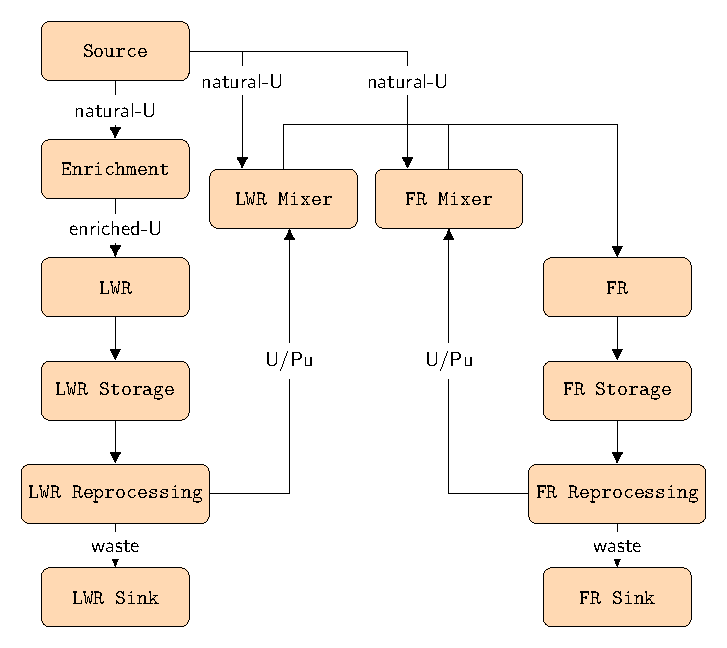
\includegraphics[width=0.45\linewidth]{../paper/figures/23flow.pdf}}
        \hspace{1em}
        \subfigure{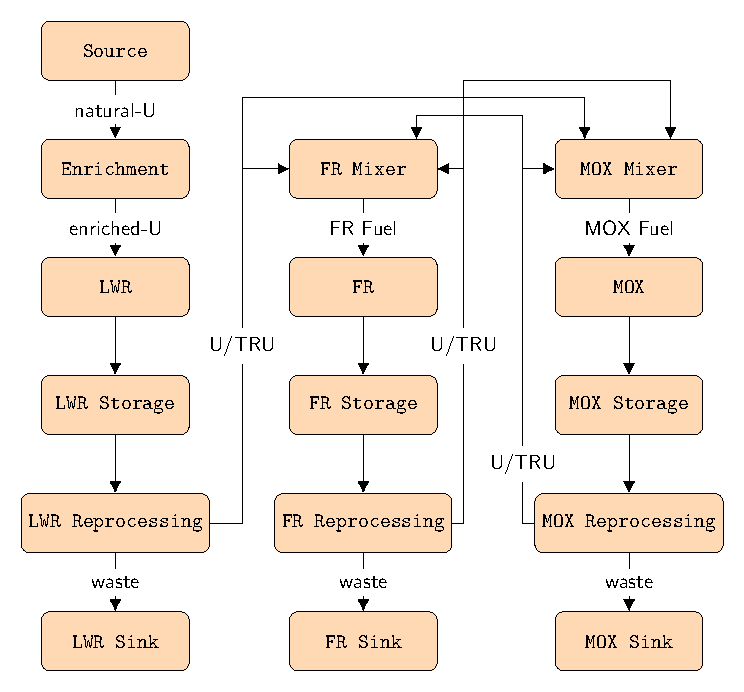
\includegraphics[width=0.45\linewidth]{../paper/figures/30flow.pdf}}
        \caption{Diagrams with facilities and mass flow of the scenarios EG01-EG23 and EG01-EG30.}
        \label{fig:eg2330}
    \end{figure}
\end{frame}